\documentclass[11pt]{article}
\usepackage{coling2020} %The coling2020 package is specific to the COLING 2020 conference (International Conference on Computational Linguistics). It defines the formatting and style guidelines required for papers submitted to that conference.
\usepackage{times} %font
\usepackage{pdfpages} %needed for hex color
\usepackage{color} %font color
\usepackage[misc]{ifsym} %for letter emoji
\usepackage{amssymb} %for symbols like \blacktriangleright
\usepackage{enumerate} %for enumerating
\usepackage[shortlabels]{enumitem} %for labels
\usepackage[cmex10]{amsmath} %for \begin{equation*}
\usepackage{amsmath,amssymb,amsfonts} %for \begin{equation*}
\graphicspath{{Figures/EPS/}{figures/}} %for \begin{split} in eqn
\usepackage[usestackEOL]{stackengine} %for \begin{split} in eqn
\usepackage{graphicx} %for figures
\graphicspath{{Figures/EPS/}{figures/}} %for figure path so that we don't have to specify the path
\usepackage{tabulary} %for picture side by side


\colingfinalcopy %The \colingfinalcopy command is a specific command provided by the coling2020 package to indicate that the document is in its final version, ready for submission. This command typically: Applies Final Formatting, Suppresses Draft-Only Features

\newcommand*{\affaddr}[1]{#1} % No op here. Customize it for different styles.

\DeclareMathOperator*{\argmin}{\arg\!\min} 
\DeclareMathOperator*{\argmax}{\arg\!\max}

\title{Workshop on LaTex for Academic, Technical, and Professional Writing}

\author{Student(Student ID: )\\
 Department of Computer Science and Engineering\\
 \affaddr{University of Chittagong, Chittagong, Bangladesh}\\
 {\tt name@gmail.com(\Letter)}\\
}

\begin{document}
\maketitle
\pagestyle{plain}

\section{Inline Text Manipulation} %The \section{Inline Text Manipulation} command creates a new section titled "Inline Text Manipulation," The title "Inline Text Manipulation" will appear in the Table of Contents (if you use \tableofcontents) 
\label{ref:inlineText} %the \label{ref:inlineText} command labels this section for later reference within the document using \ref{ref:inlineText}
This is my first LaTeX document.\\

\noindent Microblog platforms such as ``twitter", \emph{sina weibo}, etc. are rapidly moving towards a platform for $\backslash{\mbox{informal}}$ $\backslash$informal user-generated information production and consumption. Among the several microblog services , \#twitter has become the most popular. The real-time nature of twitter plays an {\color{red} important role during a disaster period}, {\color[HTML]{32a852} such as earthquakes}, \textbackslash{wildfires} and so on. This is because the user-generated twitter posts during such events might be useful to serve the situational information needs ($\approx$ 59\% \& 89\%). To\_use\_underscore it is $X_{2}$ $4^{th}$ \textcopyright2021. \\

Suppose we are given a rectangle with side lengths $(x+1)$ and $(x+3)$. Then the equation $$A=x^2+4x+3$$ represents the area of the rectangle.\\


\section{Itemize and enumerate}
\label{ref:itemize}

\subsection{The General Type of Itemize}
\begin{itemize}
\item Explore the image.
\item Explore the text.
\item Explore the video.
\item Explore the sound.
\item Create the multimodal data.
\end{itemize}

\subsection{Using the Special Symbol for Item Label}
\begin{itemize}
\item[--] Explore the image.
\item[*] Explore the image.
\item[$\diamond$] Explore the text.
\item[$\blacktriangleright$] Expore the video.
\item[$\star$] Explore the sound.
\item[$\blacksquare$] Create the multimodal data.
\end{itemize}

\subsection{Numbered Type Itemize}
\begin{enumerate}
\item Explore the image.
\item Explore the text.
\item Explore the video.
\item Explore the sound.
\item Create the multimodal data.
\end{enumerate}

\subsection{English alphabetic Type Itemize (Lowercase)}
\begin{enumerate}[a]
\item Explore the image.
\item Explore the text.
\item Explore the video.
\item Explore the sound.
\item Create the multimodal data.
\end{enumerate}

\subsection{English alphabetic Type Itemize (Uppercase)}
\begin{enumerate}[A]
\item Explore the image.
\item Explore the text.
\item Explore the video.
\item Explore the sound.
\item Create the multimodal data.
\end{enumerate}

\subsection{Roman Numbered Type Itemize (Lowercase)}
\begin{enumerate}[i]
\item Explore the image.
\item Explore the text.
\item Explore the video.
\item Explore the sound.
\item Create the multimodal data.
\end{enumerate}

\subsection{Roman Numbered Type Itemize (Uppercase)}
\begin{enumerate}[I]
\item Explore the image.
\item Explore the text.
\item Explore the video.
\item Explore the sound.
\item Create the multimodal data.
\end{enumerate}

\subsection{Reducing Space between Items}
\begin{enumerate}[nosep]
\item Explore the image.
\item Explore the text.
\item Explore the video.
\item Explore the sound.
\item Create the multimodal data.
\end{enumerate}

\subsection{Reducing Space between Items and Provide Special Item Label}
\begin{enumerate}[nosep, label=*]
\item Explore the image.
\item Explore the text.
\item Explore the video.
\item Explore the sound.
\item Create the multimodal data.
\end{enumerate}

\subsection{Reducing Space between Items and Provide Romanized Item Label}
\begin{enumerate}[nosep, label=\roman*]
\item Explore the image.
\item Explore the text.
\item Explore the video.
\item Explore the sound.
\item Create the multimodal data.
\end{enumerate}

\subsection{Reducing Space between Items and Provide Numeric Item Label}
\begin{enumerate}[nosep, label=\arabic*]
\item Explore the image.
\item Explore the text.
\item Explore the video.
\item Explore the sound.
\item Create the multimodal data.
\end{enumerate}

\subsection{Adding Specific Character with Each Numeric Item Label}
\begin{enumerate}[nosep, label=B\arabic*]
\item Explore the image.
\item Explore the text.
\item Explore the video.
\item Explore the sound.
\item Create the multimodal data.
\end{enumerate}


\subsection{Numeric Item Label with Bracket}
\begin{enumerate}[nosep, label=(\arabic*)]
\item Explore the image.
\item Explore the text.
\item Explore the video.
\item Explore the sound.
\item Create the multimodal data.
\end{enumerate}


\subsection{Numeric Item Label with Dot}
\begin{enumerate}[nosep, label=\arabic*.]
\item Explore the image.
\item Explore the text.
\item Explore the video.
\item Explore the sound.
\item Create the multimodal data.
\end{enumerate}

\subsection{Alphabetic Item Label with dot}
\begin{enumerate}[nosep, label=\alph*.]
\item Explore the image.
\item Explore the text.
\item Explore the video.
\item Explore the sound.
\item Create the multimodal data.
\end{enumerate}


\subsection{Alphabetic Item Label with dot}
\begin{enumerate}[nosep, label=\Alph*.]
\item Explore the image.
\item Explore the text.
\item Explore the video.
\item Explore the sound.
\item Create the multimodal data.
\end{enumerate}

\subsection{Romanized Item Label with dot}
\begin{enumerate}[nosep, label=\roman*.]
\item Explore the image.
\item Explore the text.
\item Explore the video.
\end{enumerate}

\subsection{Romanized Item Label with dot}
\begin{enumerate}[nosep, label=\Roman*.]
\item Explore the image.
\item Explore the text.
\item Explore the video.
\item Explore the sound.
\end{enumerate}

\subsection{Circledast label}
\begin{enumerate}[label=$\circledast$]
\item Explore the image.
\item Explore the text.
\item Explore the video.
\item Explore the sound.
\end{enumerate}

\section{Mathematical Equation and Expression}
\label{ref:equation}
\begin{equation}
e_{t} = h_{t}w_{a}
\label{eqn:sampleEqn} %this eqn can be envoked using this label
\end{equation}

\begin{equation*} % the * is so that the eqn is not numbered
a_{t} = \frac{exp(e_{t})}{\sum^T_{i=1}\exp(e_{i})}
\end{equation*}

\begin{equation*}
v = \sum^T_{i=1} a_{i} h_{i}
\end{equation*}

\begin{equation*}
P(m^{(i)},n^{(i)}) = \sum^k_{j=1} 1\{n^{(i)}=j\} \log(n_j^{\thicksim(i)}) %in case of log we have to use \ in order for it not to be italic, this is standard way to write log
\end{equation*}

\begin{equation*}
\begin{split}
\mbox{Combined Span} = &Span[index[1]] \cup \\ %cup is for union
                       &Span[index[1]] \cup \\
                       &Span[index[1]] \cup
\end{split}
\end{equation*}

\begin{equation*}
\begin{split}
R_j: & \ \mbox{if}\ x_1\ \mbox{is}\ A_{j1}\ \mbox{and/or}\ ........\ x_n\ \mbox{is}\ A_{jn} \\
     & \ \mbox{then}\ Class = C_j, \ \ \ j=1, ......,N     
\end{split}
\end{equation*}

$\underset{f_i}{argmax} ((h_i, f_i))$ \\
$\underset{f_i}{\mbox{argmax}} ((h_i, f_i))$

\subsection{Nested LSTMs (NLSTMs)}
\label{ref:nestedLSTMs}
Nowadays, LSTM based deep learning models are the most popular choice for sequential tasks. In our model, we employ the state-of-the-art nested LSTMs (NLSTMs) model where the LSTM memory cells selectively read and write necessary long-term information through accessing their inner memory. Though LSTM is employing $c_t^{outer}={f_{t}}\odot{c_{t-1}+i_t}\odot{g_{t}}$ to estimate it’s outer memory cell value, NLSTMs use the concatenation $(f_t\odot{c_{t-1}},i_t\odot{g_t}) $ as an input to an inner LSTM (or NLSTM) memory cell, and set $c_t^{outer}=h_t^{inner} $ . Such mechanism helps the NLSTMs to operate on longer time-scales thus capture the
contextual information effectively.

\section{Figure Inclusion}
\label{ref:figure}

\begin{itemize}
\item Have to use figure in pdf format for scalabilty and make sure that the font is embedded in that pdf to make sure the font can be seen even if the font is not available in another pc
\item Save as pdf from pptx, while at it select `option' and select ISO
\end{itemize}


\begin{figure}[!h] % t=top of the page, b= bottom, H/!h/htb = where it is supposed to be(! for emphasizing more)
\centering % for centered figure
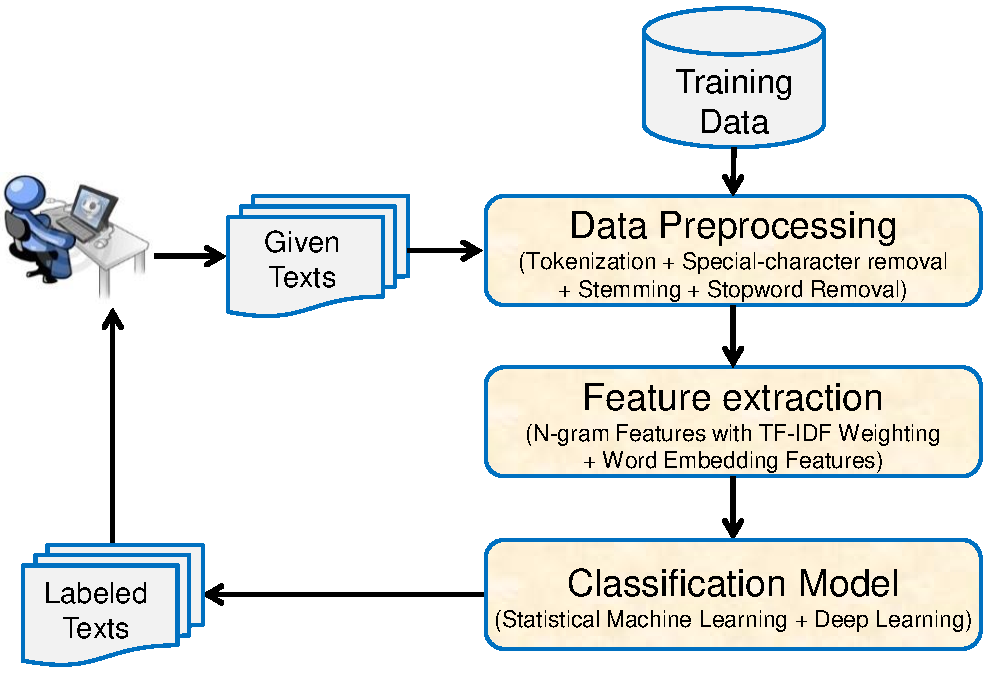
\includegraphics[width=0.7\linewidth]{ExampleSlide.pdf}
%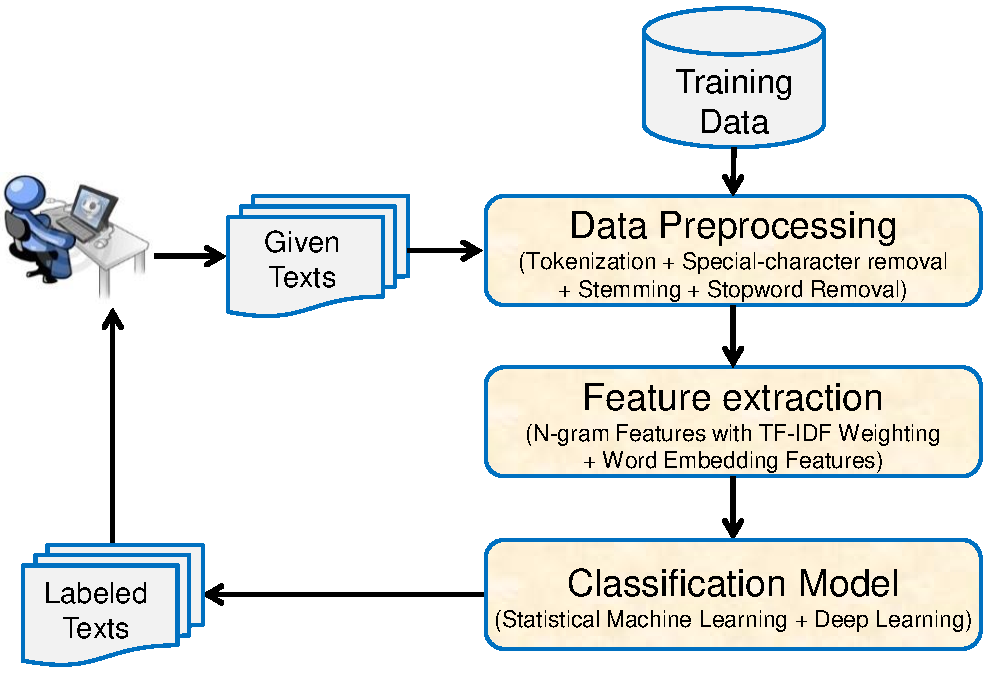
\includegraphics[scale=0.7]{ExampleSlide.pdf} also work the same
\caption{Proposed framework.}
\label{fig:overview}
\end{figure}

%\begin{figure*} here * will merge two column if the document is being wriiten in double column

\begin{figure}[!htb]
\centering
\begin{tabular}{cp{0.5cm}c}
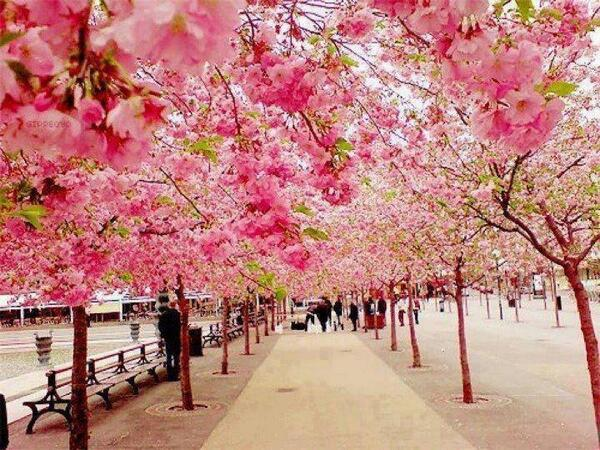
\includegraphics[width=0.4\textwidth]{Pos4.jpg}
&
&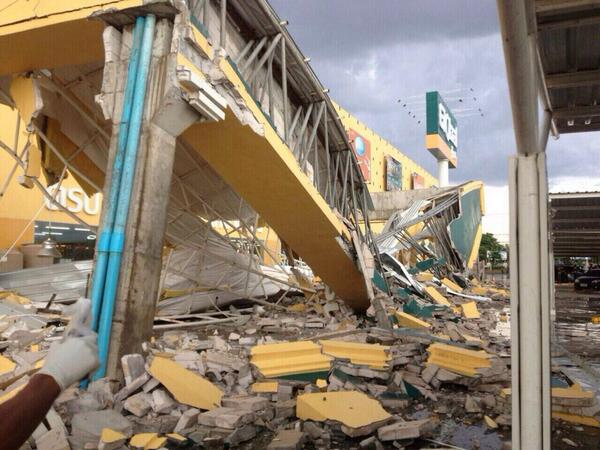
\includegraphics[width=0.4\textwidth]{Neg3.jpg}
\end{tabular}
\caption{Sample of positive (left) and negative (right) sentiment bearing images.}
\label{Fig:sampleImage}
\end{figure}

\section{Table}
\label{ref:table}
Now, we illustrate different types of tables.

\begin{table}[!htb]
\centering
\caption{A sample table.}
\begin{tabular}{|c|c|c|m{4cm}|l|c|} % c=center, l= left, these are column positions

\hline
Col1 & \textbf{Col2} & Col3 & \multicolumn{1}{c|}{Col4} & Col5 & Col6 \\
\hline
1 & 66 & 98 & 75 & 11 & 66 \\
\hline
2 & 67 & 257 & \multicolumn{1}{r|}{97} & 77 & 23 \\
\hline
\end{tabular}
\end{table}





\end{document}
